This section provides additional MarineCity visual evidence for the system
pipeline. The figures are interpreted as capture, detector, and evidence-graph
validation artifacts; quantitative detector and neural-3D scores are reported
in the main tables.

\begin{figure*}[!htbp]
\centering
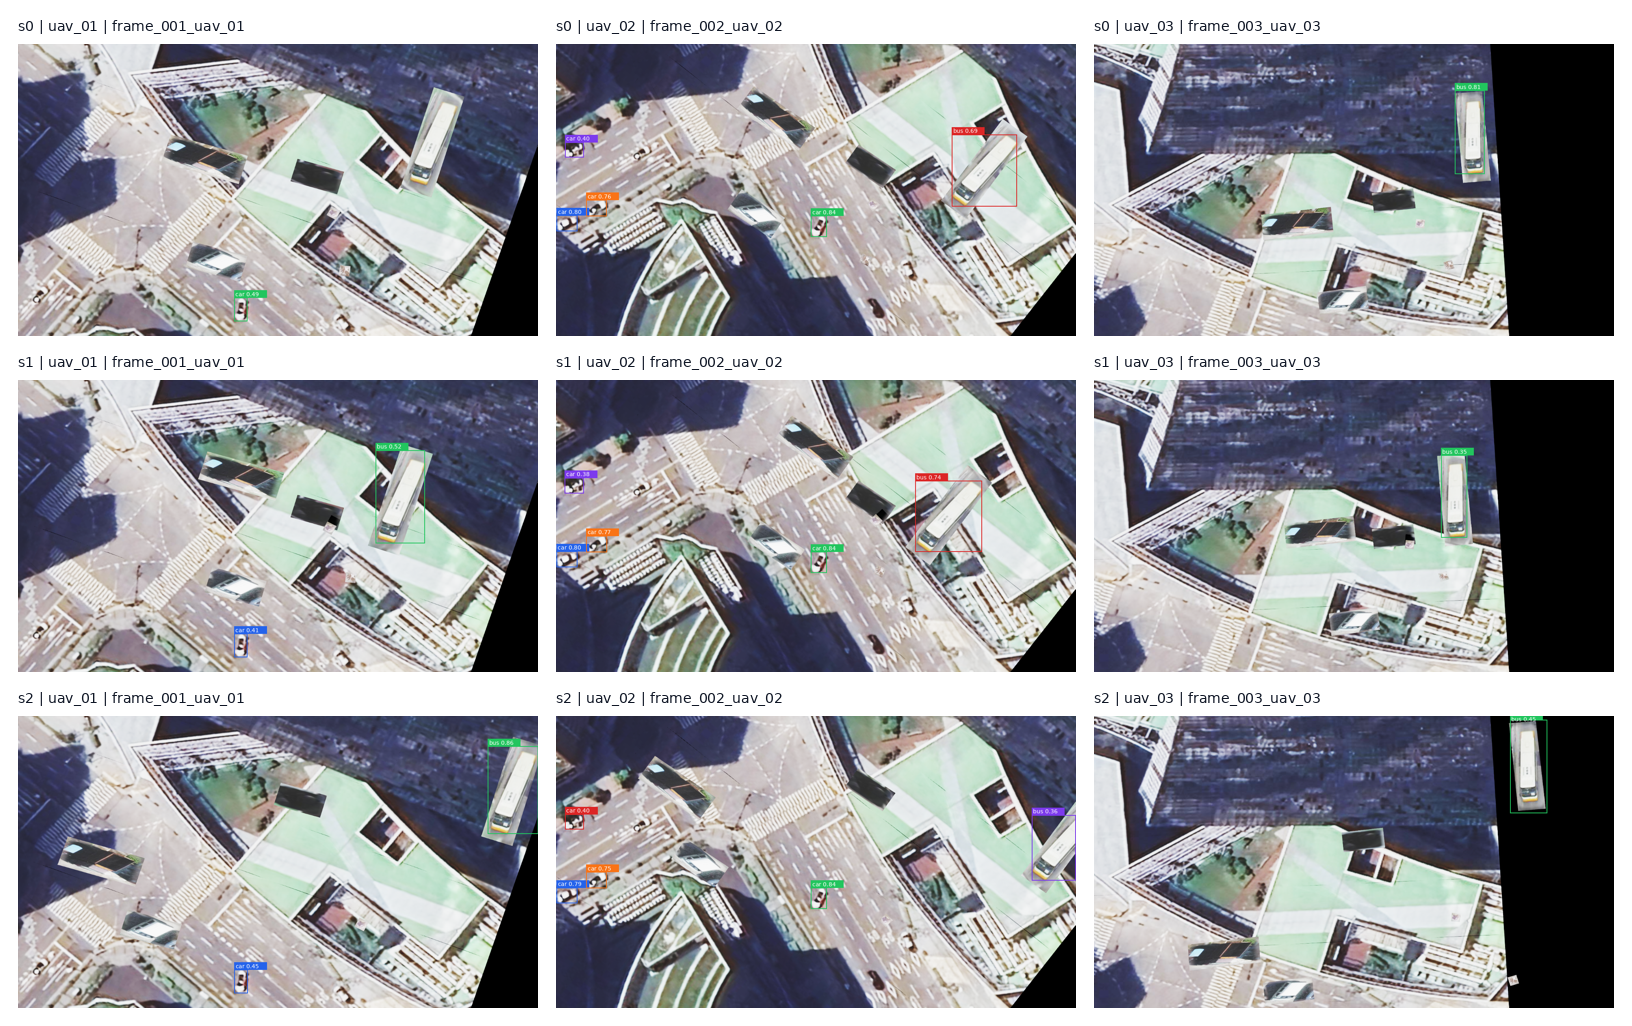
\includegraphics[width=0.98\textwidth]{figures/results/marinecity_system/marinecity_detector_preview_contact_sheet.png}
\caption{Real-Cesium MarineCity detector-to-evidence smoke-test examples. The
panels show three scenario variants and three UAV views at the verified
140--160 m camera band. Bounding boxes are produced by the current SAFR-YOLO
detector on exported real-Cesium frames and then converted into EvidenceTokens
for the 3D graph and AeroGraph validation interface. This figure validates the
capture and evidence pipeline; external-provider reasoning is reported
separately after schema-checked provider responses are imported.}
\label{fig:marinecity_detector_smoke_examples}
\end{figure*}

\begin{figure*}[!htbp]
\centering
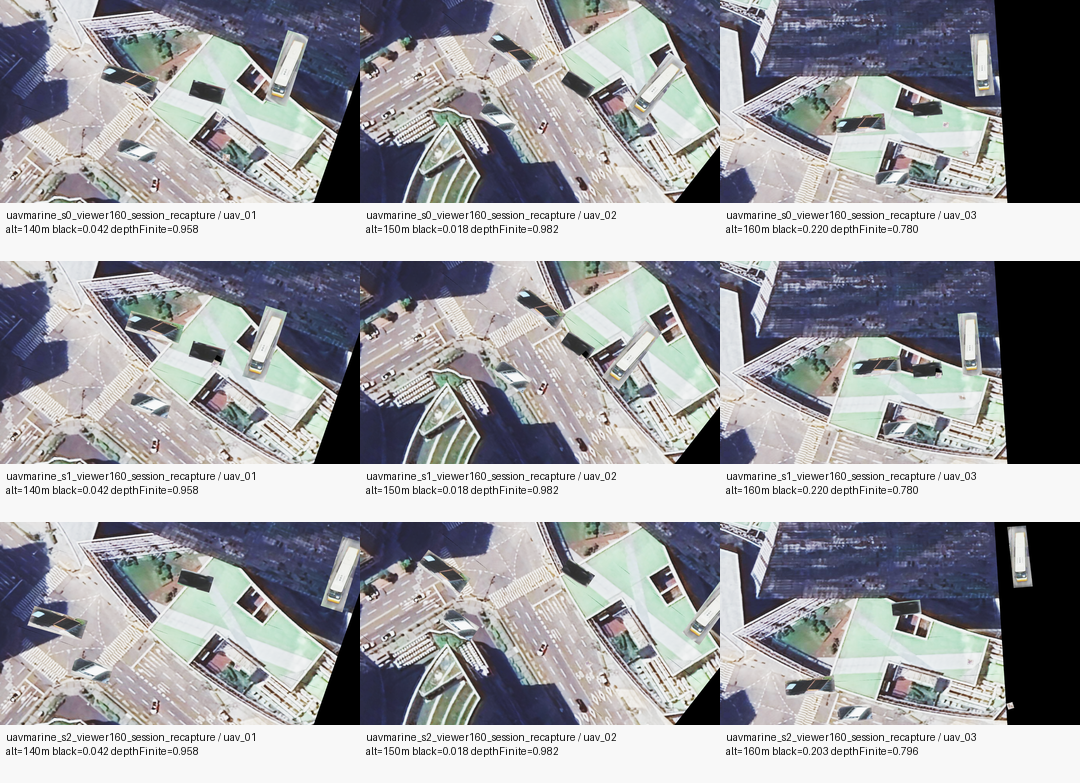
\includegraphics[width=0.98\textwidth]{figures/results/marinecity_system/marinecity_real_capture_benchmark_contact_sheet.png}
\caption{Verified real-Cesium MarineCity multi-UAV RGB capture source. The
sheet shows three scenarios and three UAV camera altitudes (140/150/160 m)
used for the current detector-to-3D evidence handoff. The black/void and
finite-depth ratios are used for qualitative figure selection; these panels are
capture evidence, not a completed NeRF/3DGS reconstruction result.}
\label{fig:supp_marinecity_real_capture_benchmark}
\end{figure*}

\begin{figure*}[!htbp]
\centering
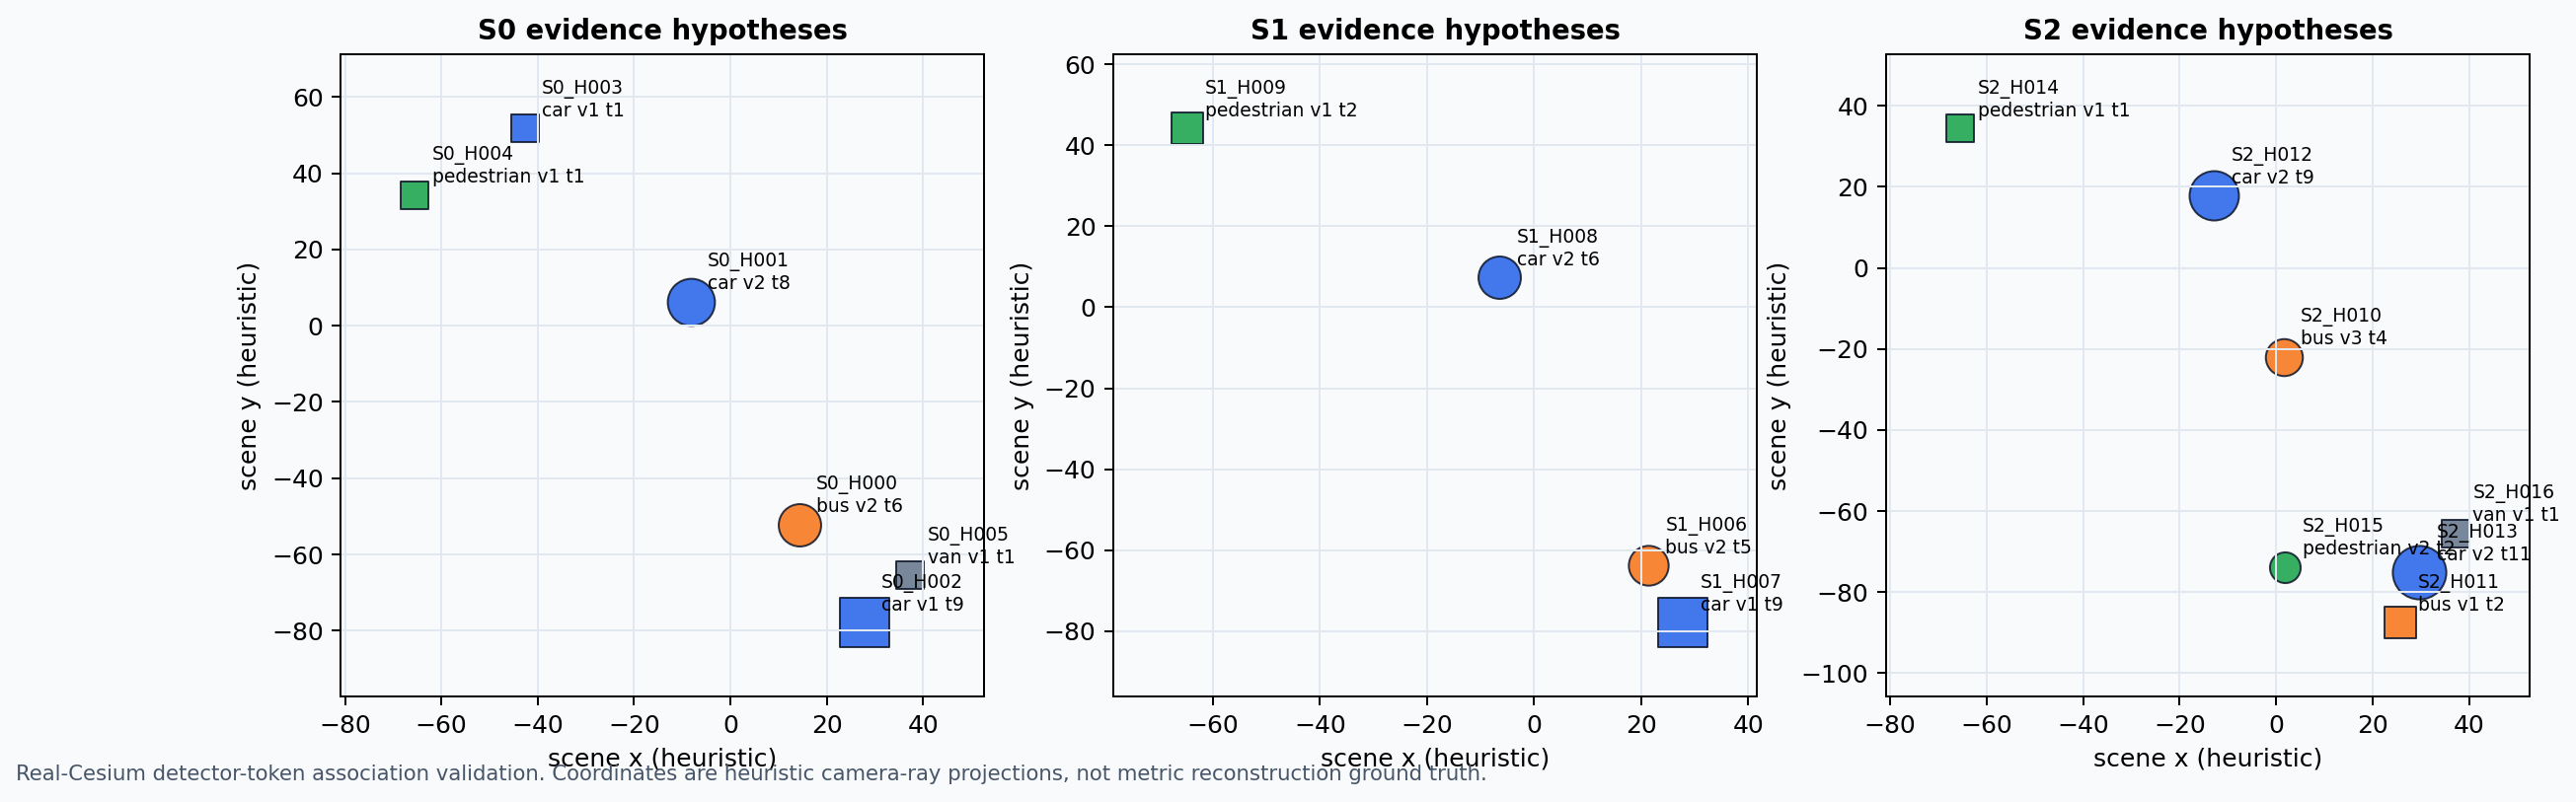
\includegraphics[width=0.98\textwidth]{figures/results/marinecity_system/marinecity_crossview_evidence_graph.png}
\caption{Real-Cesium MarineCity cross-view evidence graph smoke result. The
panels summarize heuristic camera-ray projections and support, conflict, and
missing-evidence links from the current detector EvidenceTokens. This figure is
used to validate the 2D-to-3D evidence-graph interface; it is not a metric 3D
reconstruction result.}
\label{fig:supp_marinecity_crossview_evidence_graph}
\end{figure*}

\begin{figure*}[!htbp]
\centering
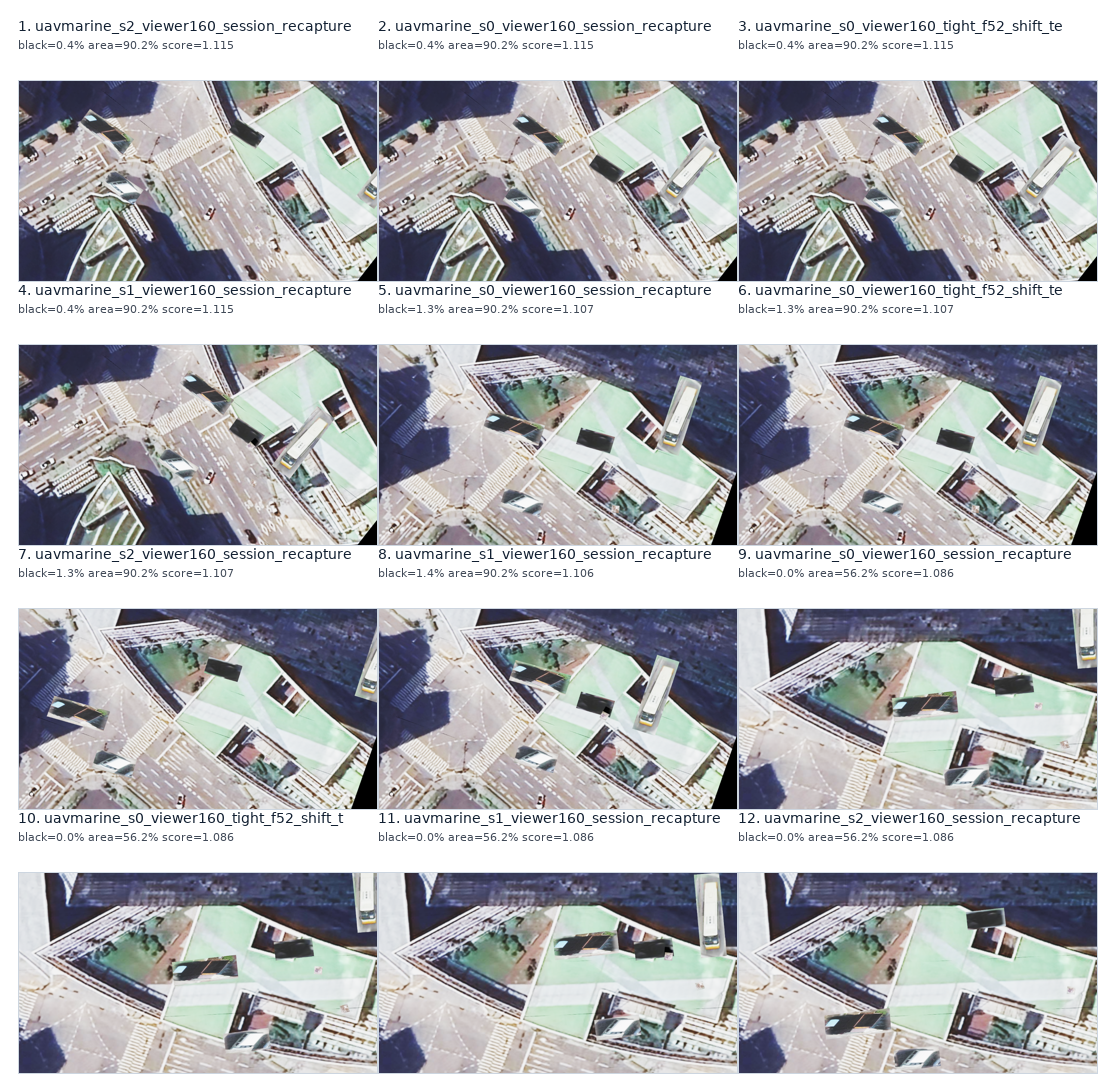
\includegraphics[width=0.98\textwidth]{figures/results/marinecity_system/marinecity_real_capture_crop_top12.png}
\caption{Real-Cesium MarineCity crop candidates used for qualitative framing.
The crops are selected from the full saved scene to show small-object regions
more clearly; they are not synthetic replacements for the capture source. The
current best crop is from the S2 viewer160 recapture, with void ratio 0.0036
and crop-only area ratio 0.9025.}
\label{fig:supp_marinecity_crop_candidates}
\end{figure*}

\begin{figure*}[!htbp]
\centering
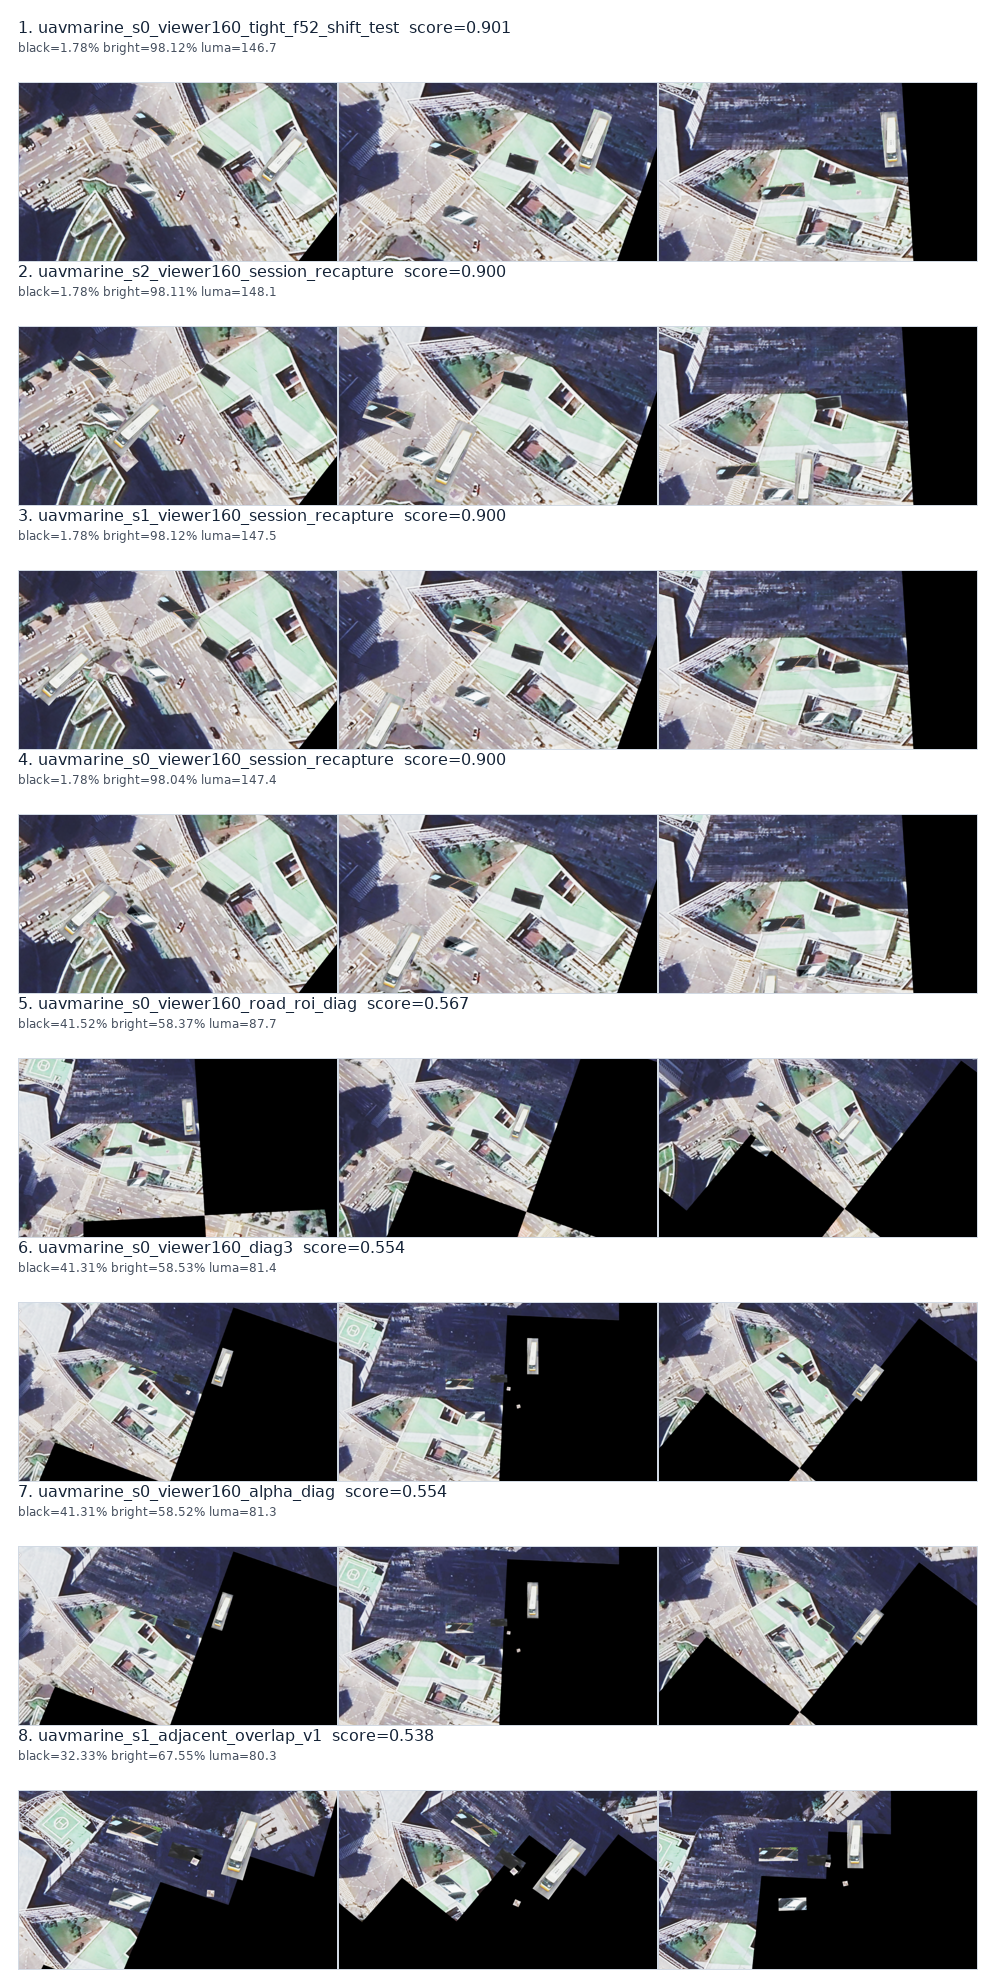
\includegraphics[width=0.98\textwidth]{figures/results/marinecity_system/marinecity_capture_quality_top8.png}
\caption{Visual quality audit for full real-Cesium MarineCity captures. The
sheet compares black/void tile regions and brightness so that qualitative
figures are chosen from the clearest real-Cesium captures. The current best
full-capture candidate is the S2 viewer160 recapture, with mean top-3 void
ratio 0.0876.}
\label{fig:supp_marinecity_capture_quality}
\end{figure*}

\paragraph{MarineCity qualitative analysis.}
These supplementary figures separate four visual checks that are easy to
conflate in the main paper. Fig.~\ref{fig:marinecity_detector_smoke_examples}
checks whether the detector-to-token export works on real-Cesium UAV views.
Fig.~\ref{fig:supp_marinecity_real_capture_benchmark} verifies the capture
source and altitude band, while
Fig.~\ref{fig:supp_marinecity_crossview_evidence_graph} shows that the saved
tokens can be grouped into support, conflict, and missing-evidence links.
Figs.~\ref{fig:supp_marinecity_crop_candidates} and
\ref{fig:supp_marinecity_capture_quality} are used for figure selection and
failure auditing; they are not additional quantitative claims.
